\printconcepts
\exercise{T/F: The Product Rule states that $\ds \frac{d}{dx}\big(x^2\sin x\big) = 2x\cos x$.
}{F
}

\exercise{T/F: The Quotient Rule states that $\ds \frac{d}{dx}\left(\frac{x^2}{\sin x}\right) = \frac{2x}{\cos x}$.}{F}

\exercise{T/F: The derivatives of the trigonometric functions that start with ``c'' have minus signs in them.
}{T
}

\exercise{What derivative rule is used to extend the Power Rule to include negative integer exponents?
}{Quotient Rule
}

\exercise{T/F: Regardless of the function, there is always exactly one right way of computing its derivative.
}{F
}

\exercise{In your own words, explain what it means to make your answers ``clear.''
}{Answers will vary.
}

%\exercise{Give an example of a function where $\fp(x) \neq 0$ and $\fpp(x) = 0$.}{One possible answer is $f(x) = 17x-205$.}

%\exercise{Explain in  your own words what the second derivative ``means.''}{Answers will vary.}

%\exercise{If $f(x)$ describes a position function, then $\fp(x)$ describes what kind of function? What kind of function is $\fpp(x)$?}{$\fp(x)$ is a velocity function, and $\fpp(x)$ is acceleration.}

%\exercise{Let $f(x)$ be a function measured in pounds, where $x$ is measured in feet. What are the units of $\fpp(x)$?}{lbs/ft$^2$.}

\printproblems
\exerciseset{In Exercises}{, use the Quotient Rule to verify these derivatives.
}{

\exercise{$\dfrac{d}{dx}(\cot x) = -\csc^2 x$}{\begin{align*}
\frac{d}{dx}(\cot x)
&=\frac{d}{dx}\left(\frac{\cos x}{\sin x}\right)\\
&=\frac{\sin x (-\sin x) - (\cos x)(\cos x)}{(\sin x)^2}\\
&=\frac{-[(\sin x)^2 + (\cos x)^2]}{(\sin x)^2}\\
&=\frac{-1}{(\sin x)^2} = -\csc^2 x
\end{align*}}

\exercise{$\dfrac{d}{dx}(\sec x) = \sec x \tan x$}{\begin{align*}
\frac{d}{dx}(\sec x)
&=\frac{d}{dx}\left(\frac{1}{\cos x}\right)\\
&=\frac{\cos x \cdot 0 - 1 \cdot (-\sin x)}{(\cos x)^2}\\
&=\frac{\sin x}{(\cos x)^2} = \sec x \tan x
\end{align*}}

\exercise{$\dfrac{d}{dx}(\csc x) = -\csc x \cot x$}{\begin{align*}
\frac{d}{dx}(\csc x)
&=\frac{d}{dx}\left(\frac{1}{\sin x}\right)\\
&=\frac{\sin x \cdot 0 - 1 \cdot (\cos x)}{(\sin x)^2}\\
&=\frac{-\cos x}{(\sin x)^2} = -\csc x \cot x
\end{align*}}

}
\input{exercises/02_04_exset_01}
\exerciseset{In Exercises}{:
\begin{enumerate}
\item[(a)] Use the Quotient Rule to differentiate the function.
\item[(b)] Manipulate the function algebraically and differentiate without the Quotient Rule.
\item[(c)] Show that the answers from (a) and (b) are equivalent.
\end{enumerate}
}{

\exercise{$\ds f(x)= \frac{x^2+3}{x}$
}{\begin{enumerate}
\item		$\fp(x) = \frac{x(2x)-(x^2+3)1}{x^2}$
\item		$\fp(x) = 1-\frac{3}{x^2}$
\item		They are equal.
\end{enumerate}
}

\exercise{$\ds g(x)= \frac{x^3-2x^2}{2x^2}$
}{\begin{enumerate}
\item		$g'(x) = \frac{2x^2(3x^2-4x)-(x^3-2x^2)(4x)}{4x^4}$
\item		$g'(x) = 1/2$
\item		They are equal.
\end{enumerate}
}

\exercise{$\ds h(s)= \frac{3}{4s^3}$
}{\begin{enumerate}
\item		$h'(s) = \frac{4s^3(0) - 3(12s^2)}{16s^6}$
\item		$h'(s) = -9/4s^{-4}$
\item		They are equal.
\end{enumerate}
}

\exercise{$\ds f(t)= \frac{t^2-1}{t+1}$
}{\begin{enumerate}
\item		$\fp(t) = \frac{(t+1)(2t) - (t^2-1)(1)}{(t+1)^2}$
\item		$f(t) = t-1$ when $t\neq -1$, so $\fp(t) = 1$.
\item		They are equal.
\end{enumerate}
}
}
%\ifthenelse{\boolean{printquestions}}{\columnbreak}{}
\input{exercises/02_04_exset_03}
\input{exercises/02_04_exset_04}
\exerciseset{In Exercises}{, find the $x$-values where the graph of the function has a horizontal tangent line.}{

\exercise{$f(x) = 6x^2-18x-24$}{$x=3/2$}

\exercise{$f(x) = x\sin x$ on $[-1,1]$}{$x=0$}

\exercise{$\ds f(x) = \frac{x}{x+1}$}{$\fp(x)$ is never 0.}

\exercise{$\ds f(x) = \frac{x^2}{x+1}$}{$x= -2,0$}

}

\begin{exerciseset}{In Exercises}{, find the requested derivative.}

\exercise{$f(x) = x\sin x$; find $\fpp(x)$.}{$\fpp(x) = 2\cos x - x\sin x$}

\exercise{$f(x) = x\sin x$; find $f\,^{(4)}(x)$.}{$f^{(4)}(x) = -4\cos x+ x\sin x$}

\exercise{$f(x) = \csc x$; find $\fpp(x)$.}{$\fpp(x) = \cot^2x\csc x + \csc^3 x$}

\exercise{$f(x) = (x^3-5x+2)(x^2+x-7)$; find $f\,^{(8)}(x)$.}{$f^{(8)} = 0$}

\end{exerciseset}

%\ifthenelse{\boolean{printquestions}}{\columnbreak}{}
{\noindent In Exercises}
{, $f$ and $g$ are differentiable functions such that $f(2)=3$, $\fp(2)=-1$, $g(2)=-5$, and $g'(2)=2$. Evaluate the expressions.
}
\exinput{exercises/02_04_ex_61}
\exinput{exercises/02_04_ex_62}
\exinput{exercises/02_04_ex_63}
\exinput{exercises/02_04_ex_64}
\exinput{exercises/02_04_ex_65}
\exinput{exercises/02_04_ex_66}

\exercise{If $f$ and $g$ are functions whose graphs are shown, evaluate the expressions.\\
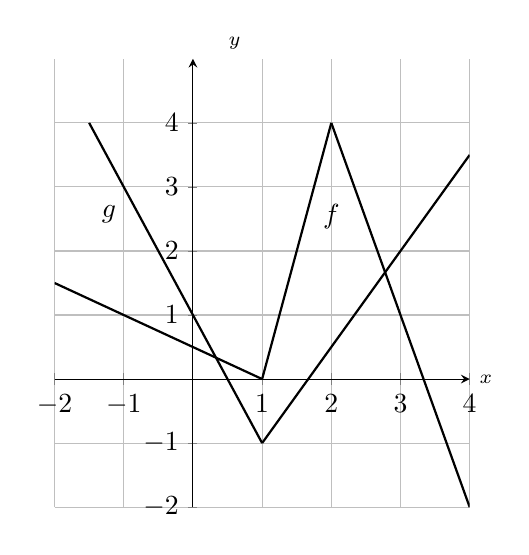
\begin{tikzpicture}
\begin{axis}[axis y line=middle,axis x line=middle, ymajorgrids=true, xmajorgrids=true, ymin=-2,ymax=5, xmin=-2,xmax=4, name=myplot, xscale=1/1.3, ytick={-2,-1,0,1,2,3,4}]
\addplot [{\colorone}, domain=-1.5:1,thick] {-2*x+1}; 
\addplot [{\colorone}, domain=1:4,thick] {1.5*x-2.5};
\addplot [{\colortwo}, domain=-2:1, thick] {-.5*x+.5};
\node[label={30:{$g$}}] at (axis cs:-1.6,2.2) {};
\addplot [{\colortwo}, domain=1:2, thick] {4*x-4};
\node[label={30:{$f$}}] at (axis cs:1.6,2.1) {};
\addplot [{\colortwo}, domain=2:4, thick] {-3*x+10};
\end{axis}
\node [right] at (myplot.right of origin) {\scriptsize $x$};
\node [above] at (myplot.above origin) {\scriptsize $y$};
\end{tikzpicture}\\*
\begin{tabular}{ll}
(a) $(fg)'(-1)$  & (b) $(f/g)'(-1)$ \\
(c) $(fg)'(3)$ & (d) $(g/f)'(3)$
\end{tabular}}{(a) $-\frac{7}{2}$ (b) $\frac{1}{8}$ (c) $-\frac{9}{2}$ (d) $\frac{15}{2}$}

\exerciseset{In Exercises}{, use the graph of $f(x)$ to sketch $\fp(x)$.}{

\exercise{\begin{minipage}[]{\linewidth}
\myincludegraphics[scale=.8]{figures/fig02_04_ex_43}
\end{minipage}
}{\mbox{}\\[-\baselineskip]\myincludegraphics[scale=.8]{figures/fig02_04_ex_43a}
}

\exercise{\begin{minipage}[]{\linewidth}
\myincludegraphics[scale=.8]{figures/fig02_04_ex_44}
\end{minipage}
}{\mbox{}\\[-\baselineskip]\myincludegraphics[scale=.8]{figures/fig02_04_ex_44a}
}

\exercise{\begin{minipage}[]{\linewidth}
\myincludegraphics[scale=.8]{figures/fig02_04_ex_45}
\end{minipage}
}{\mbox{}\\[-\baselineskip]\myincludegraphics[scale=.8]{figures/fig02_04_ex_45a}
}

}


%\printreview

%\exercise{Given that $e^0=1$, approximate the value of $e^{0.1}$ using the tangent line to $f(x) = e^x$ at $x=0$.}{The tangent line to $f(x) = e^x$ at $x=0$ is $y=x+1$; thus $e^{0.1} \approx y(0.1) = 1.1$. }

%\exercise{Approximate the value of $(3.01)^4$ using the tangent line to $f(x) = x^4$ at $x=3$.}{The tangent line to $f(x) = x^4$ at $x=3$ is $y=108(x-3)+81$; thus $(3.01)^4 \approx y(3.01) = 108(.01)+81 = 82.08$. }
